% Hero figure: the one idea the whole library is built on.
% A residual-stream state h projected onto the reward direction w_r.
% The reward is that projection (plus bias); the dashed line is a level set r = const.
% Compile with ../build_figures.sh -> content/assets/figures/reward-projection.svg
\documentclass[border=10pt]{standalone}
\usepackage{tikz}
\usetikzlibrary{calc,arrows.meta}
\definecolor{rlink}{HTML}{3F51B5}    % reward direction
\definecolor{raccent}{HTML}{FF5722}  % the readout
\definecolor{rmuted}{HTML}{6B7280}
\begin{document}
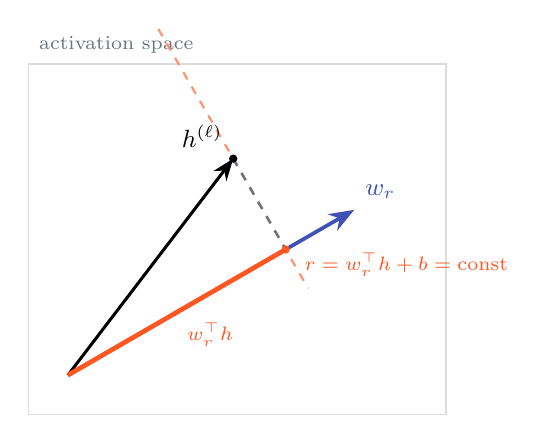
\begin{tikzpicture}[>=Stealth, line width=0.9pt, font=\small]
  \coordinate (O) at (0,0);
  \coordinate (W) at (30:4.2);
  \coordinate (H) at (2.1,2.75);
  \coordinate (F) at ($ (O)!(H)!(W) $);

  % faint activation-space frame
  \draw[rmuted!25, line width=0.6pt] (-0.5,-0.5) rectangle (4.8,3.95);
  \node[rmuted, font=\scriptsize, anchor=south west] at (-0.5,3.95) {activation space};

  % level set of constant reward, perpendicular to w_r, through h
  \draw[raccent!65, dashed, line width=0.8pt]
     ($ (H) + (120:1.9) $) -- ($ (H) + (-60:1.9) $);
  \node[raccent, font=\scriptsize, anchor=west] at ($ (H) + (-60:1.55) $)
     {$r = w_r^{\top} h + b = \mathrm{const}$};

  % reward direction
  \draw[rlink, ->, line width=1.35pt] (O) -- (W)
     node[above right, rlink] {$w_r$};

  % a residual-stream state at some layer
  \draw[->, line width=1.1pt] (O) -- (H) node[above left] {$h^{(\ell)}$};

  % orthogonal drop onto the reward axis
  \draw[rmuted, dashed] (H) -- (F);

  % the reward readout: how far h reaches along w_r
  \draw[raccent, line width=1.7pt] (O) -- (F);
  \node[raccent, font=\scriptsize, anchor=north west] at ($ (O)!0.5!(F) $)
     {$w_r^{\top} h$};

  \fill (H) circle (1.5pt);
  \fill[raccent] (F) circle (1.5pt);
\end{tikzpicture}
\end{document}
